% Chapter 3

\chapter{Data Integration} % Chapter title

\label{ch:dataintegration} % For referencing the chapter elsewhere, use \autoref{ch:mathtest}
%----------------------------------------------------------------------------------------
%
%----------------------------------------------------------------------------------------
\section{The Datasets}
\subsection{Australian Water Availability Project}
As mentioned in \autoref{subsection:dataavailability} \nameref{subsection:dataavailability}, the Australian Water Availability Project (AWAP) is a joint effort contributed by CSIRO Marine and Atmospheric Research (CMAR), the Bureau of Meteorology (BoM) and the Bureau of Rural Science (BRS)\citep{Raupach2009}.\\
\newline
The AWAP aims to contribute to the overall understanding and monitoring of the Australian landscape systems, particularly the changes and feedback in climate, so that proper and robust management can be applied on a system-scale. It monitors the state and trend of the terrestrial water balance of the Australian continent.\\
\newline 
The approach it takes is based on model-data fusion, which is combining information from both the models and the data to maximise knowledge about the system. It contains historic and up-to-date data of soil moisture and all water influx and efflux contributing to changes in soil moisture (rainfall, transpiration, soil evaporation, surface runoff and deep drainage etc.), across Australia at a spatial resolution of 5 km. \\
\newline 
The AWAP data is available for access through a web interface, it provides three forms: (1) weekly near-real-time reporting, (2) historical monthly time series (1900 to present), and (3) monthly climatologies.\\
\begin{figure}[hbt]
\myfloatalign
\subfloat[{Precipitaion[mm/d]}]
{\label{fig:awapprec1}
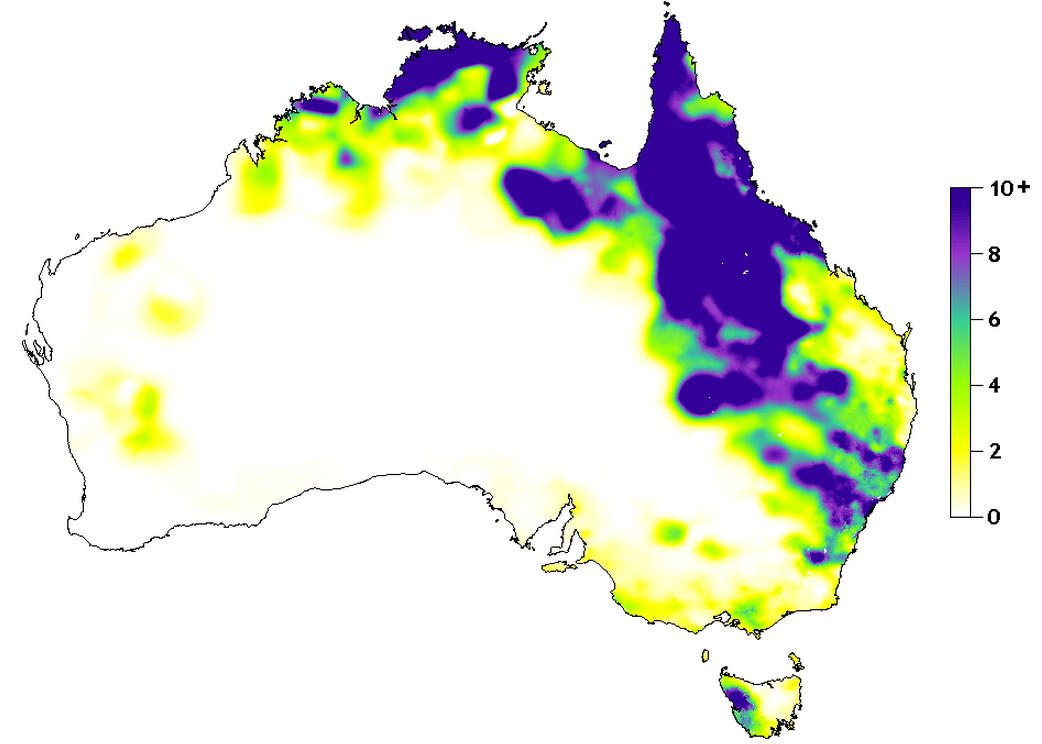
\includegraphics[width=.45\linewidth]{gfx/awapprec}} \quad
\subfloat[{Percent Rank Precipitaion[\%]}]
{\label{fig:awapprec2}
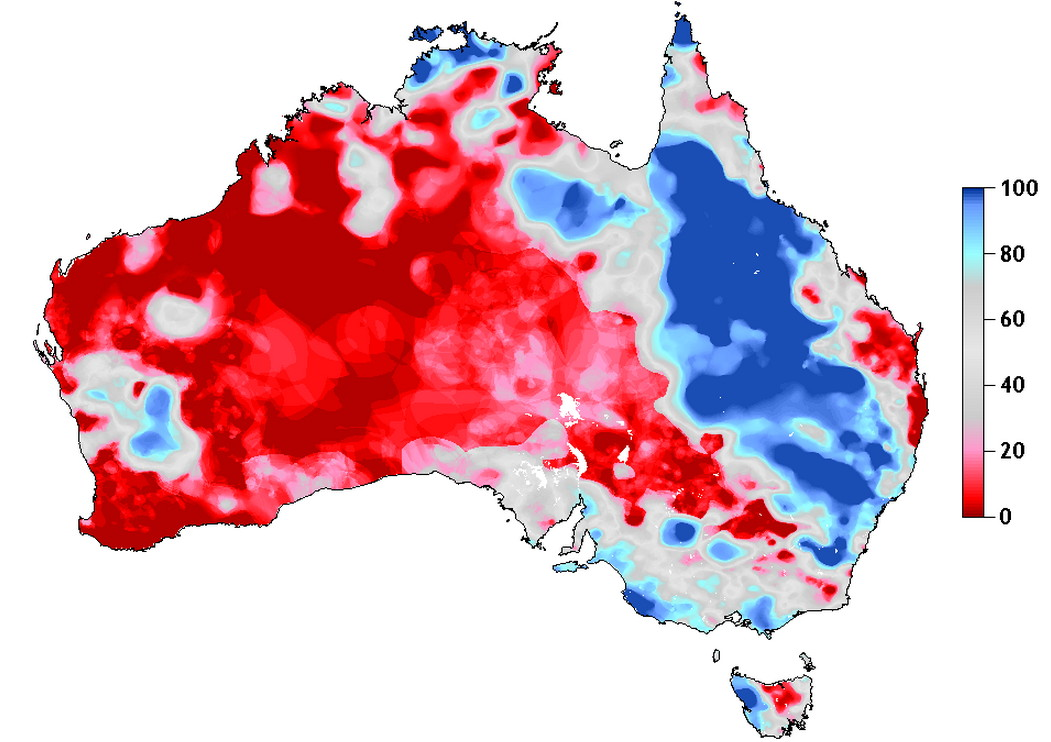
\includegraphics[width=.45\linewidth]{gfx/awapprecper}}
\caption{Example of AWAP weekly near-real-time data. Date: 2014/02/17 to 2014/02/23. Acquired from CSIRO\citep{Awap2014}.}
\label{fig:awapprec}
\end{figure}
\newline
\autoref{fig:awapprec} shows an example of AWAP weekly data acquired from the web interface hosted by CSIRO. The example displays the precipitaion data in both physical values(\autoref{fig:awapprec1}) and percentage rank(\autoref{fig:awapprec2}) of the week from 2014/02/17 to 2014/02/23 on the Australian territories.
\subsection{CosmOz: Australian National Cosmic Ray Soil Moisture Monitoring Facility} 
The Australian National Cosmic Ray Soil Moisture Monitoring Facility(CosmOz) is a near-real-time soil moisture measurement network provided by CSIRO, Monash University, Charles Darwin University and the University of New South Wales\citep{cosmoz2014}. it aims to test the utility of cosmic ray sensor system for water management, water information and hydrological process research applications, as well as to test the feasibility and utility of a national near-real time soil moisture measurement network. CosmOz also supports the evaluation of remote sensing products and hydrological models by expanding the set of soil moisture data available over Australia.\\
\newline
CosmOz currently has deployed 13 sensor systems at 12 locations across Australia, shown in \autoref{fig:cosmozloc}. Each CosmOz sensor system includes: 1* Hydroinnova CRS-1000 cosmic ray soil moisture sensor, 1* Hydrological Services tipping-bucket rain gauge, 3* Campbell TDR soil moisture probes and Quaesta data logger with integrated Iridium SBS satellite data communications.
\begin{figure}[hbt]
\myfloatalign
\subfloat[{Location of the 12 CosmOz monitoring sites. Acquired from University of Arizona\citep{arizona2014}}]
{\label{fig:cosmozloc}
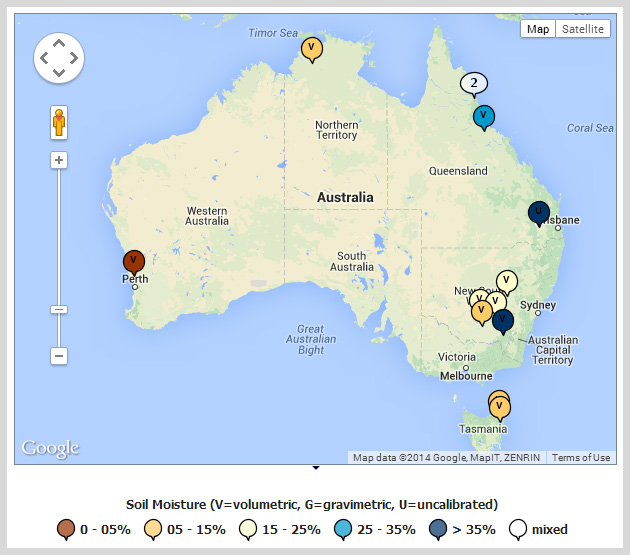
\includegraphics[width=.52\linewidth]{gfx/cosmozloc}} \quad
\subfloat[{CosmOz system installed at Tullochgorum in Tasmania. Reprinted from ``{C}osm{O}z {W}iki Page'', by \citeauthor{cosmoz2014}, 2013. Copyright 2013 by \citeauthor{cosmoz2014}.}]
{\label{fig:cosmozphoto}
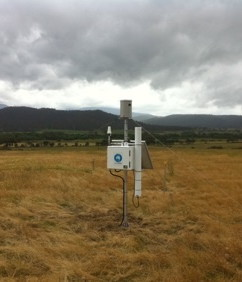
\includegraphics[width=.39\linewidth]{gfx/cosmozphoto}}
\caption{The Australian National Cosmic Ray Soil Moisture Monitoring Facility(CosmOz) and one of its probes deployed in Tullochgorum site.}
\label{fig:cosmoz}
\end{figure}

\subsection{Landsat program}
The Landsat program is a joint effort of the U.S. Geological Survey (USGS) and the National Aeronautics and Space Administration (NASA). The lantsat satellites have continuously acquired and delivered images of the Earth's land surface since 1972\citep{Mission2013}. The Landsat satellites have provided a valuable archive of space-based land remotely sensed data, contributed greatly in the studies of agriculture, geology, forestry, education, region planning, mapping and global change research.\\
\begin{figure}[bth]
\begin{center}
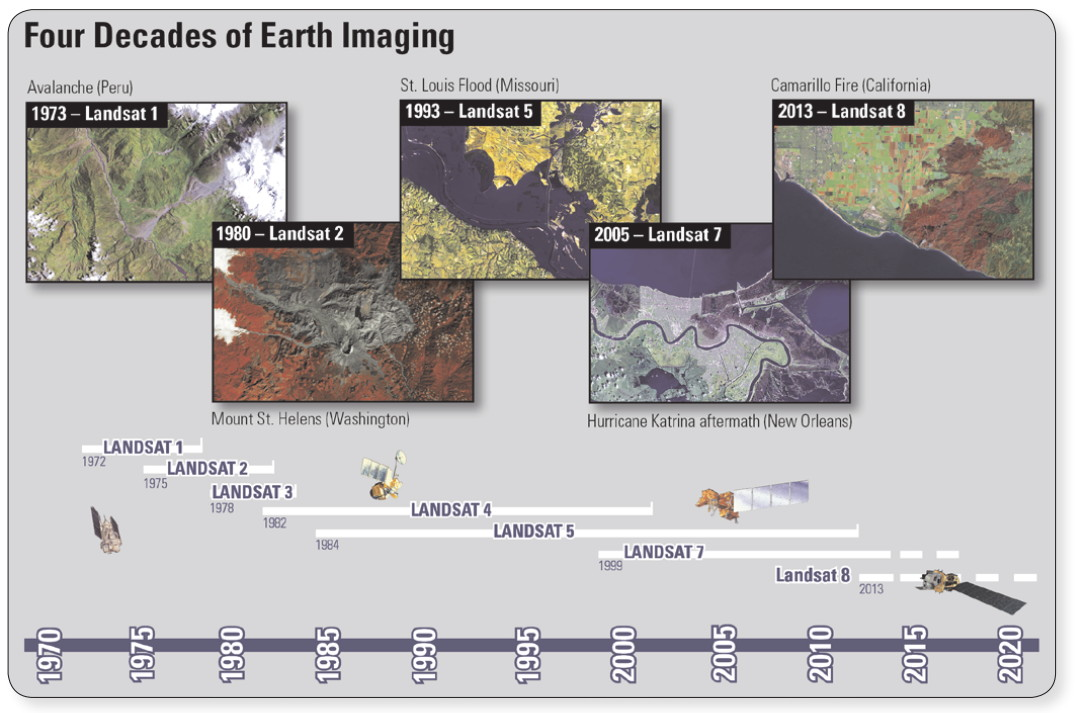
\includegraphics[width=.95\linewidth]{gfx/landsat}
\end{center}
\caption{Overview of the Landsat program. Reprinted from ``Landsat: A Global Land-Imaging Mission'', by USGS, 2013. Copyright 2013 by USGS.  }
\label{fig:landsat4decades}
\end{figure}
\newline
Landsat 8 is the eighth and the latest Landsat satellite, launched on 11 February 2013. \autoref{table:landsatsum} details the eight Landsat satellites in terms of launch/decommission time, operation status and the sensors on-board respectively. In the ``Sensors'' column, Landsat 1,2,3 carries Multispectral Scanner (MSS) and Return Beam Vidicon Camera (RBV), Landsat 4,5 carries MSS and Thematic Mapper (TM), Landsat 6 carries Enhanced Thematic Mapper (ETM), Landsat 7 carries Enhanced Thematic Mapper Plus (ETM+) and Landsat 8 carries Operational Land Imager (OLI) and Thermal Infrared Sensor (TIRS).\\
\begin{table}[hbt]
\caption{Details of Landsat missions. Adapted from ``Landsat: A Global Land-Imaging Mission'', by USGS, 2013. Copyright 2013 by USGS.}
\begin{center}
\rowcolors{2}{cyan!15}{white} 
\begin{tabular}{llll} 
\hline
\textbf{Satellite}&\textbf{Launch}&\textbf{Decommissioned}&\textbf{Sensors}\\
\hline
Landsat 1 & 23 July 1973 & 6 January 1978 & MSS/RBV \\
Landsat 2 & 22 January 1975 & 27 July 1983 & MSS/RBV \\
Landsat 3 & 5 March 1978 & 7 Septermber 1983 & MSS/RBV \\
Landsat 4 & 16 July 1982 & 15 July 2001 & MSS/TM \\
Landsat 5 & 1 March 1984 & 2013 & MSS/TM \\
Landsat 6 & 5 October 1993 & Did not achieve orbit & ETM\\
Landsat 7 & 15 April 1999 & Operational & ETM+ \\
Landsat 8 & 11 February 2013 & Operational & OLI/TIRS\\
\hline 
\end{tabular}
\end{center}
\label{table:landsatsum}
\end{table}
\newline
It is noteworthy that both Landsat 6 and Landsat 7 suffered from operational failures. Landsat 6 did not achieve its target orbit during launching procedure, thus it was officially declared as a failure by the National Oceanic and Atmospheric Administration (NOAA)\citep{Viets1995}. Landsat 7 experienced a failure in its Scan Line Corrector (SLC) mechanism, which resulted in wedge-shaped scan-to-scan gaps. As shown in \autoref{fig:l7slcoff} comparing to \autoref{fig:l7slcon}, there are blank gaps on the image where data is not available.
\begin{figure}[hbt]
\myfloatalign
\subfloat[{Landsat 7 Natural Color Image with SLC-ON. Captured on 9 January 2003.}]
{\label{fig:l7slcon}
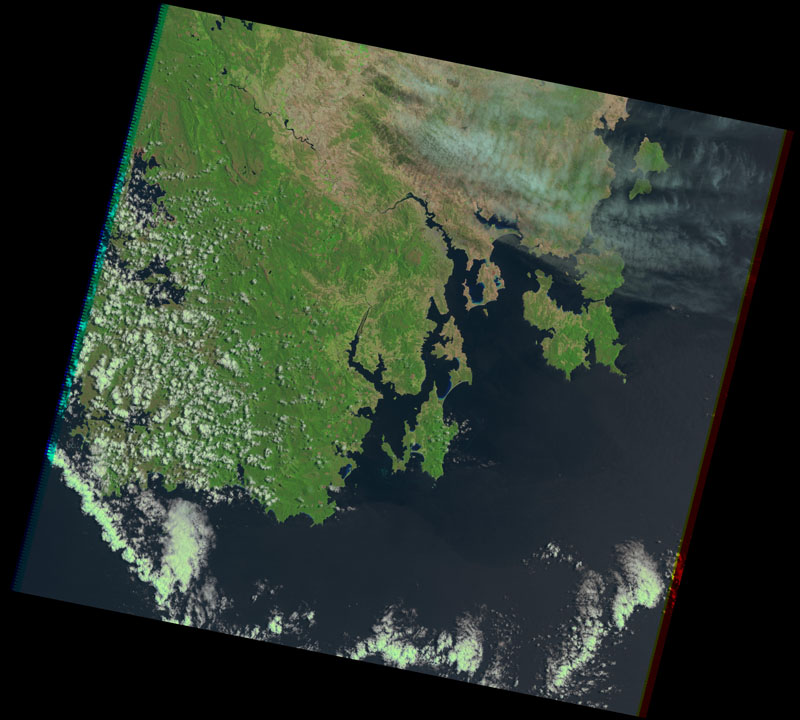
\includegraphics[width=.45\linewidth]{gfx/l7slcon}} \quad
\subfloat[{Landsat 7 Natural Color Image with SLC-OFF (with gaps). Captured on 25 March 2007.}] 
{\label{fig:l7slcoff}
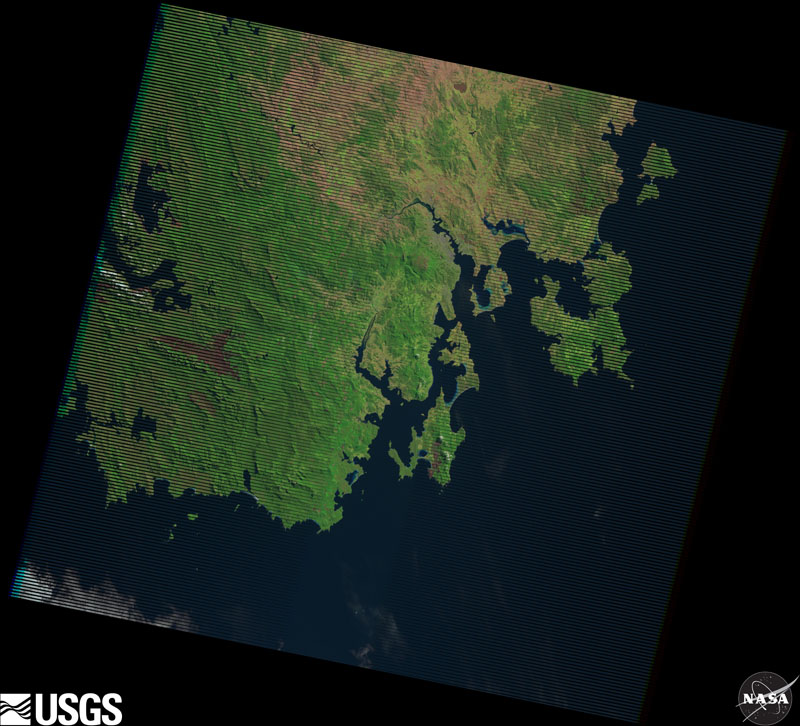
\includegraphics[width=.45\linewidth]{gfx/l7slcoff}}
\caption{Landsat 7 ETM+ images of the Tasmania south-eastern area captured before and after the SLC failure. Acquired from USGS.}
\label{fig:l7slc}
\end{figure}

\subsection{Moderate-resolution Imaging Spectroradiometer}

\subsection{National Elevation Data Framework}

\subsection{SILO}

